\section{Introduction}

The Geophysics Department of the University of Helsinki uses a SQUID 
magnetometer for measuring the magnetism of rocks and meteorites. There is 
already a program for using the machine, but its usability could be better. The 
source code of the existing program is available.

The goal of this project is to improve the existing program by making a better 
user interface for it. A secondary goal is to link the measurements produced by 
the program to desired after-processing programs.

The project will take place from 25.1.2005 to 6.5.2005.


\section{Organization}

The people related to this project are shown in Figure~\ref{fig:organization}.

\begin{figure}[h]
\begin{tabular}{llll}
{\bf Name} & {\bf Role} & {\bf E-Mail} & {\bf Phone} \\
\hline
Mikko Jormalainen	& Project Team	& mtjormal@cc.helsinki.fi		& 040 545 6249 \\
Samuli Kaipiainen	& Project Team	& samuli.kaipiainen@cs.helsinki.fi	& 050 357 0359 \\
Aki Korpua		& Project Team	& aki.korpua@cs.helsinki.fi		& 044 339 5375 \\
Esko Luontola		& Project Team	& esko.luontola@cs.helsinki.fi		& 041 507 1474 \\
Aki Sysm�l�inen		& Project Team	& aki.sysmalainen@helsinki.fi		& 0400 603 416 \\
\hline
Lauri J. Pesonen	& Client	& lauri.pesonen@helsinki.fi		& \\
Tomas Kohout		& Client	& tomas.kohout@helsinki.fi		& \\
Fabio Donadini		& Client	& fabio.donadini@helsinki.fi		& \\
\hline
Juha Taina		& Course manager	& taina@cs.helsinki.fi		& 09 191 51311 \\
Jenni Valorinta		& Instructor		& valorint@cs.helsinki.fi	& 09 191 51165, \\
			&			&				& 040 540 2846
\end{tabular}
\caption{The people who are part of this project}
\label{fig:organization}
\end{figure}


\subsection{Responsibilities}

The responsibilities of the project team members are described here. The 
assignments are shown in Figure~\ref{fig:responsibilities}.

\begin{figure}[h]
\begin{tabular}{ll}
{\bf Responsibility} & {\bf Person} \\
\hline
Project Manager		& Esko Luontola \\
Secretary		& Mikko Jormalainen, Samuli Kaipiainen, \\
			& Aki Korpua, Aki Sysm�l�inen \\
CVS Manager		& Aki Korpua \\
HTML Manager		& Esko Luontola \\
Measurement Manager	& Aki Sysm�l�inen \\
\hline
Project Plan		& Esko Luontola \\
Requirements Document	& Aki Sysm�l�inen, Aki Korpua \\
Design Document		& Mikko Jormalainen, Samuli Kaipiainen \\
Testing Plan		& Aki Korpua, Mikko Jormalainen \\
Testing Report		& Aki Korpua, Mikko Jormalainen \\
User Manual		& Aki Sysm�l�inen, Samuli Kaipiainen \\
Realization Document	& Aki Sysm�l�inen, Samuli Kaipiainen \\
Final Report		& Esko Luontola
\end{tabular}
\caption{Assigned responsibilities}
\label{fig:responsibilities}
\end{figure}

{\bf Project Manager} \\
Is responsible for leading the project team. Writes the project plan and takes 
care that the project progresses according to it.

{\bf Secretary} \\
The secretary changes every week. Writes the meeting records and forwards them 
to the team.

{\bf CVS Manager} \\
Sets up the CVS system and takes care of it during the project. Guides others in 
the use of CVS.

{\bf HTML Manager} \\
Updates the web site and adds the published documents there.

{\bf Measurement Manager} \\
Takes the measurements that are gathered from OHTU projects and submits them to 
the course manager.


% \newpage
\section{General Description of the Product}

The SQUID magnetometer is used for measuring the magnetism of rocks and 
meteorites. The machine consists of three main components: measurement unit, 
demagnetizing unit and sample holder. The computer guides their operation 
through COM ports. The existing source code will be used to control the machine 
on a low level, and on top of it will be built a new user interface.

The program must be able to control the machine, gather measurements from the 
samples, show them to the user and save the results on disk for later use. The 
program will be used on a modern PC running Windows. The old program has been 
written in Visual C. The new program will be written either in C and Java, or in 
C++.

The name of the program will be Ikayaki (dried, grilled squid - a Japanese 
seafood).


\section{Estimated Size}

The size of the old source code is about 12,000 lines of code. Taking into 
account, that part of the old source will be reused, and that the new program 
will be more complex than the old one, it can be estimated that we will need to 
write about 10,000 lines of code (+-30\%). A better estimation will be made when 
the program requirements are known better.


\section{Workflow}

The process of developing this program is described here. There are two 
concurrent processes: one for finding out the program requirements and building 
the user interface, and one for finding out how the source code works and 
building an application interface for using the SQUID.

\subsection{Main Process: GUI and producing the program}

The process for creating the new user interface will follow a linear waterfall 
model. The output of the previous phase will be the input of the next one.

\subsubsection{Definition}

Requirements analysis will be done with the client and the program requirements 
will be listed. The client will guide the project team in using the existing 
program and magnetometer. The results will be requirements document and user 
interface prototype. The client will accept the documents before proceeding.

\subsubsection{Design}

The user interface and structure of the program will be designed. The expertise 
of the client will be needed during this phase. Designing will be made so 
accurately that producing the program will be as simple as possible. The results 
will be design document and testing plan. The client will accept the documents 
before proceeding.

\subsubsection{Production}

The program will be written according to the design document. Each programmer 
will take care of the unit testing of his own code. The result will be program 
code.

\subsubsection{Testing}

The program will be tested according to the test plan and the found errors will 
be corrected. Uncorrected errors will be documented. User manual will be 
written. The results will be testing report, user manual and realization 
document.

\subsubsection{Installing}

The program will be given to the client and the project team will install it in 
the laboratory. Possibly an installer will be created for wider distribution. 
Documentations will be tweaked and final report written.


\subsection{Sub Process: analyzing the old source code}

Analyzing the old source code, designing a suitable interface for using the 
SQUID and building it will be executed concurrently with the main process. The 
interface needs to be defined before the main process will need the information 
in its design phase.

The sub process will utilize 1-2 persons.

\subsubsection{Design}

Getting to know the old source code and finding out how the program works. An 
interface for using the magnetometer will be designed. The result will be 
interface design document and testing plan, which will be attached to the actual 
design document and testing plan.

\subsubsection{Production}

The interface will be built according to the design plan.

\subsubsection{Testing}

The interface will be tested with real equipment according to the test plan. If 
the interface is completed much before the user interface is ready, it might be 
necessary to build a simple user interface for testing purposes only. Otherwise 
the interface will be tested with the rest of the program.

\subsection{Schedule}

The length of the project is about 14 weeks, starting 25.1.2005 and ending 
latest 6.5.2005. The lengths of the phases are shown in 
Figure~\ref{fig:schedule}. They are also described graphically using a GANTT 
diagram in Figure~\ref{fig:schedulegantt}.

\begin{figure}[h]
\begin{tabular}{lllll}
{\bf Task} & {\bf Start} & {\bf End} & {\bf Days} & {\bf Results} \\
\hline
Project Plan		& 25.1.2005	& 15.2.2005	& 21	& Project Plan \\
Definition		& 25.1.2005	& 22.2.2005	& 28	& Requirements Document, Prototype \\
(Main) Design		& 22.2.2005	& 15.3.2005	& 21	& Design Document, Testing Plan \\
(Sub) Design		& 25.1.2005	& 22.2.2005	& 28	& (Design Document, Testing Plan) \\
(Main) Production	& 15.3.2005	& 29.3.2005	& 14	& Program Code \\
(Sub) Production	& 22.2.2005	& 1.3.2005	& 7	& Program Code \\
(Main) Testing		& 29.3.2005	& 26.4.2005	& 28	& Testing Report, User Manual, \\&&&& Realization Document \\
(Sub) Testing		& 1.3.2005	& 22.3.2005	& 21	& (Testing Report) \\
Installing		& 26.4.2005	& 3.5.2005	& 7	& Final Report
\end{tabular}
\caption{Project schedule}
\label{fig:schedule}
\end{figure}

\begin{figure}
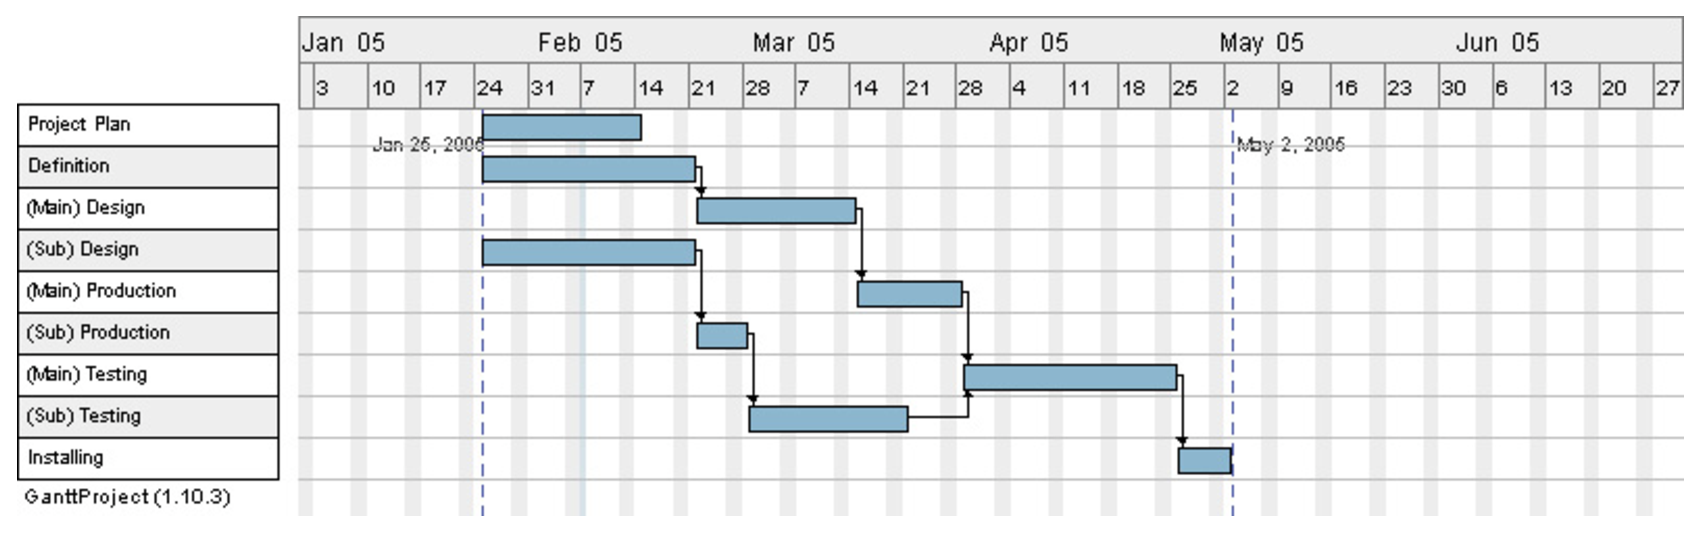
\includegraphics[width=15cm]{aikataulu.eps}
\caption{Project schedule as a GANTT diagram}
\label{fig:schedulegantt}
\end{figure}

% Kuvaa, miten projekti jakaantuu pienempiin osiin. Osien v�lisi� suhteita on 
% syyt� selvent�� ns. GANTT-kaavion avulla. Aikataulua laadittaessa kannattaa 
% ottaa huomioon kaikki mahdolliset ennalta tiedett�v�t tapahtumat, esimerkiksi 
% eri tuotosten er�p�iv�t, seurantakokousten p�iv�m��r�t, projektiryhm�n j�senten 
% mahdolliset poissaolot, kaikille projekteille yhteinen demotilaisuus jne.
% 
% Kun aikataulun esitt�� tarkasti, projektin seuranta on helppoa. Osallistujien 
% v�lisen ty�njaon voi esitt�� t�ss�.


\section{Conventions}

Meetings will be held every Tuesday at 10-12 and Thursday at 10-12 in Exactum 
class A219. The secretary will write a record and publish it as soon as possible 
after the meeting.

Every meeting should have a pre-made list of the items that need to be discussed 
in that meeting. If somebody won't be able to make it to a meeting, he should 
report it beforehand. The items should be discussed in an orderly manner and an 
item needs to be completed before moving to the next one. Documents that will be 
handled in a meeting must be published the day before the meeting before 18:00.

Work sessions will be held on Wednesdays at 14-18 when necessary. The team will 
meet in the Exactum lobby by default.

Communication outside the meetings will be through e-mail and the mailing list 
ohtuk05-squid-list@cs.helsinki.fi. All e-mail messages should be prefixed with 
(squid). The project has an IRC channel \#squid-project at IRCnet.

The material produced in the project will be managed with CVS. The CVSROOT is \\ 
/home/group/squid/.cvsroot

Every team member should write what he is doing currently to a text file so that 
it could be viewed from the web site: \\ 
/group/home/squid/public\_html/username/status.txt

The team uses the locker 1 in room A307.


\section{Documentation}

During the project the following documents will be published. They will be made 
with LaTeX and published in PDF format. Documents will be stored in the CVS 
during the project.

\begin{itemize}
\item Project plan
\item Requirements Document
\item Design Document
\item Testing Plan
\item User Manual
\item Testing Report
\item Final Report
\item Realization Document
\item Meeting Records (in Finnish)
\end{itemize}


\section{Risk Analysis}

\subsection{Team}

{\bf Risk:} Communication in a foreign language causes problems. \\
{\bf Propability:} Low \\
{\bf Seriousness:} Medium \\
{\bf Countermeasures:} Those who known English better, will be used to 
communicate with the client.

{\bf Risk:} A team member gets sick. \\
{\bf Propability:} Medium \\
{\bf Seriousness:} Medium \\
{\bf Countermeasures:} The rest of the team should be informed as soon as 
possible, so that others can share the work when necessary.

{\bf Risk:} A team member quits the project. \\
{\bf Propability:} Low \\
{\bf Seriousness:} High \\
{\bf Countermeasures:} Maintain a happy and encouraging atmosphere.


\subsection{Project Management}

{\bf Risk:} The estimations (size of work, skills) are incorrect. \\
{\bf Propability:} High \\
{\bf Seriousness:} Medium \\
{\bf Countermeasures:} Keep and eye on the project plan and update it as 
necessary.

{\bf Risk:} The project will not stay in schedule. \\
{\bf Propability:} High \\
{\bf Seriousness:} High \\
{\bf Countermeasures:} Look at the schedule at the end of every week to notice 
problems as soon as possible. Adjust the schedule when necessary. Drop secondary 
features off the program (do not neglect testing!).

{\bf Risk:} The project will not be completed in time. \\
{\bf Propability:} Medium \\
{\bf Seriousness:} High \\
{\bf Countermeasures:} If the program appears too big for us to complete it, 
produce only the core elements of it, but do them well. It is possible that some 
other team will then continue from where we were left.

{\bf Risk:} Communication is not adequate. \\
{\bf Propability:} Medium \\
{\bf Seriousness:} Medium \\
{\bf Countermeasures:} Arrange regular meetings between the team members. Follow 
closely what everybody is doing at the moment and what the results are.

{\bf Risk:} Participants are not interested in the project. \\
{\bf Propability:} Low \\
{\bf Seriousness:} High \\
{\bf Countermeasures:} Keep everybody informed about the status of the project 
to keep their interest up. Show the current results for the client when there is 
something to show. Arrange interesting work for the team members.

{\bf Risk:} Some personal interest takes the time of a team member. \\
{\bf Propability:} Medium \\
{\bf Seriousness:} Medium \\
{\bf Countermeasures:} Follow closely what everybody is doing. If somebody does 
not show progress, find out what is wrong. Tell others if you know that you will 
not have enough time.


\subsection{Technology}

{\bf Risk:} The old source code and the operation of the machine is not being 
understood well enough, and there will be problems in the reuse of the code.  \\
{\bf Propability:} Medium \\
{\bf Seriousness:} High \\
{\bf Countermeasures:} Allocate more people to have a look at the source code. 
Discard the old source and start from a scratch, if the inclusion of legacy code 
proves to be too risky.

{\bf Risk:} The SQUID gets broken. \\
{\bf Propability:} Low \\
{\bf Seriousness:} High \\
{\bf Countermeasures:} Test the code well before trying it with the real machine.

{\bf Risk:} If some need to learn a new programming language, their code will 
have more bugs and they will write it slower. \\
{\bf Propability:} High \\
{\bf Seriousness:} Medium \\
{\bf Countermeasures:} Utilize the existing knowledge of the individuals as much 
as possible. Try coding in pairs. Do thorough testing. Make one or two people 
learn the new stuff well, so that others won't need to spend as much time on it.

{\bf Risk:} If some need to learn using new tools, they will be slow in using them. \\
{\bf Propability:} Medium \\
{\bf Seriousness:} Low \\
{\bf Countermeasures:} Take the learning curve into consideration and adjust the 
schedule. Make one or two people learn the new stuff well, so that others won't 
need to spend as much time on it.

{\bf Risk:} A person is not skilled enough in the task that has been assigned to him. \\
{\bf Propability:} Low \\
{\bf Seriousness:} Low \\
{\bf Countermeasures:} Assign that person to do some other work where he is 
better. Try to utilize the special skills of the team members as much as 
possible, especially in case of a difficult task.


\subsection{Client}

{\bf Risk:} The project team will not understand how the magnetometer is being used. \\
{\bf Propability:} Medium \\
{\bf Seriousness:} High \\
{\bf Countermeasures:} Check all decisions concerning the program design with 
the client. Build an accurate prototype of the system and make the client accept 
it before writing code. 

{\bf Risk:} The client you tried to contact can not be reached. \\
{\bf Propability:} Low \\
{\bf Seriousness:} Medium \\
{\bf Countermeasures:} Find out beforehand if the client knows when he will be 
unavailable. Try to do other things that do not require the client while 
waiting. They to become independent of the client after the beginning of the 
project.

{\bf Risk:} The client will not be satisfied with the finished product or the 
product will be useless. \\
{\bf Propability:} Medium \\
{\bf Seriousness:} High \\
{\bf Countermeasures:} Build prototypes and write documents that will be 
accepted by the client. Test the program thoroughly.

{\bf Risk:} The client does not understand the prosess of making software. \\
{\bf Propability:} High \\
{\bf Seriousness:} Low \\
{\bf Countermeasures:} Explain to the client what we are doing. Remind the 
client not to expect too much.


% \section{Muuta muistettavaa}
% 
% Sopivissa kohdissa projektisuunnitelmaa voi ottaa kantaa seuraaviin
% asioihin.
% 
% \begin{itemize}
% \item Laadunvalvonta projektin aikana.
% \item Projektin kriittinen polku.
% \item Tarkastukset ja katselmukset.
% \item Sihteerivuorot, jos sihteerin teht�v� on kiert�v�.
% \item Yhteenveto tuotettavista dokumenteista.
% \item Yhteenveto muista osatuotoksista, jos niit� on.
% \item Asiakkaan vastuulla olevat asiat.
% \end{itemize}
